\chapter{Approach}


% Describe the performed solution with all possible details. Define necessary parameters, inputs, outputs and context of use, possible problems and when they can be applied. 

% Remember to define necessary concepts before using them, building the text from easiest definitions (not depending on previous definitions) to complex definitions (depending on previous definitions).

% E.g: 
% \begin{itemize}
%	\item Lost Communication: a lost communication occurs when the conditions of the environment are not sufficient or the distance between sender and receiver is to hight to transmit information.
%	\item Wait until rescue: when the robot loses its communication, the pre-designed state machine will stop the motors to keep the actual position. Energy safe mode will be enabled, at the same time that a channel transceiver daemon will send SOS messages every T and wait for reply during T sec. 
%\end{itemize}

The challenge is how to coordinate multiple robots to execute a set of tasks. To tackele this problem, a communication efficient scheduler system is designed, where each robot autonomously request task from the centralized scheduler and centralized scheduler response with a set of suitable tasks. The architecture of this centralized scheduler is shown in Figure \ref{fig:system_architecture}.


\begin{figure}[htbp]
	\centering
	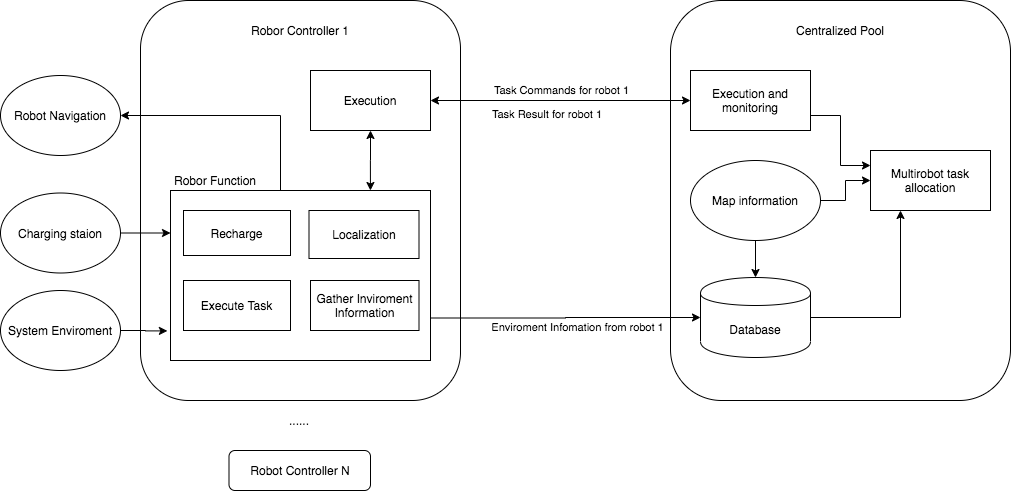
\includegraphics[width = 0.6\textwidth]{content/images/ch3/architecture.drawio.png}
	\caption{System architecture}
	\label{fig:system_architecture}
\end{figure}

\section{The System Components}


\subsection{Robot Components}


\begin{figure}[htbp]
	\centering
	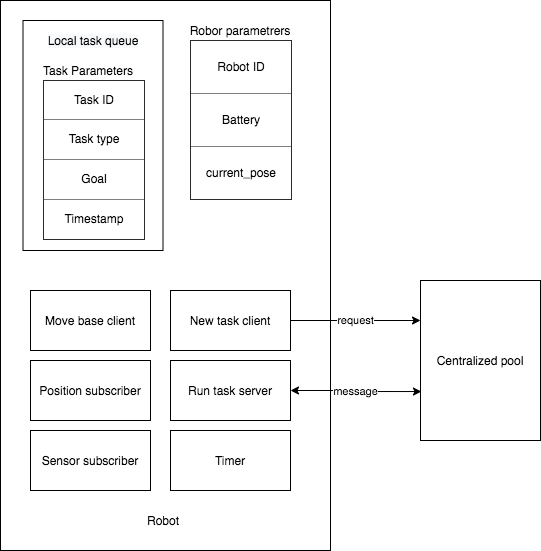
\includegraphics[width = 0.45\textwidth]{content/images/ch3/system_component_robot.drawio.png}
	\caption{Robot Components}
	\label{fig:robot_components}
\end{figure}

\begin{itemize}
	\item \textsl{Robot ID.} Robot ID is a unique identification for each robot.
	\item \textsl{Battery level.} Battery level drops as the robot moves and rotates.
	\item \textsl{Task type.} Robots perform different tasks such as "Charging", " Execute Task", "Gather Enviroment Information". For details please refer to Section \ref{sec:task_types}
	\item \textsl{Local task queue.} Local task queue keeps a list of tasks that a robot will run sequentially. Once a task is finished, it would be removed from task queue. Once this queue become empty, the robot send task result to centralized pool.
	\item \textsl{New task client.} Once all task are finished, the new task client send request to new task server.
	\item \textsl{Run task server.} The run task server receive tasks and send task feedback and task result.
	\item \textsl{Timer.} To prevent robot to be hanged by one task forever, the timer check the robot moving state periodically.
	\item \textsl{Move base client.} The move\_base node provides a ROS interface for configuring, running, and interacting with the navigation stack on a robot. The move\_base client send a goal to move\_base node to tracking their status  
	\item \textsl{Position subscriber.} The position subscriber get robot current position from navigation stack. The robot send its current location to centralized pool to request a new task.
	\item \textsl{Sensor subscriber.} The Sensor subscriber listen to sensor data within the range.
\end{itemize}

\subsection{Centralized Pool Components}

\begin{figure}[htbp]
	\centering
	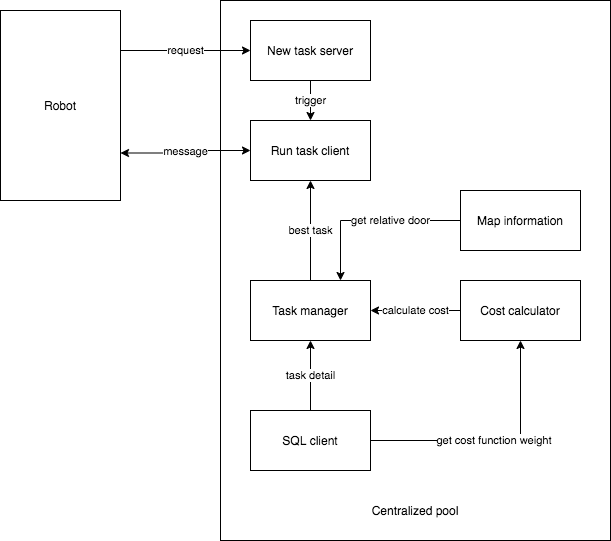
\includegraphics[width = 0.45\textwidth]{content/images/ch3/system_component_centralized_pool.drawio.png}
	\caption{Centralized Pool Components}
	\label{fig:centralized_pool_components}
\end{figure}

\begin{itemize}
	\item \textsl{Map Information.} Map information contains information such as the door list that the robot will pass through when moving to target position.
	\item \textsl{Cost calculator.} Cost calculator calculate the cost for doors, rooms and charging stations.
	\item \textsl{Task manager.} Task manager can construct, sort and allocate tasks.
\end{itemize}


\section{Communication Protocols}

\begin{figure}[htbp]
	\centering
	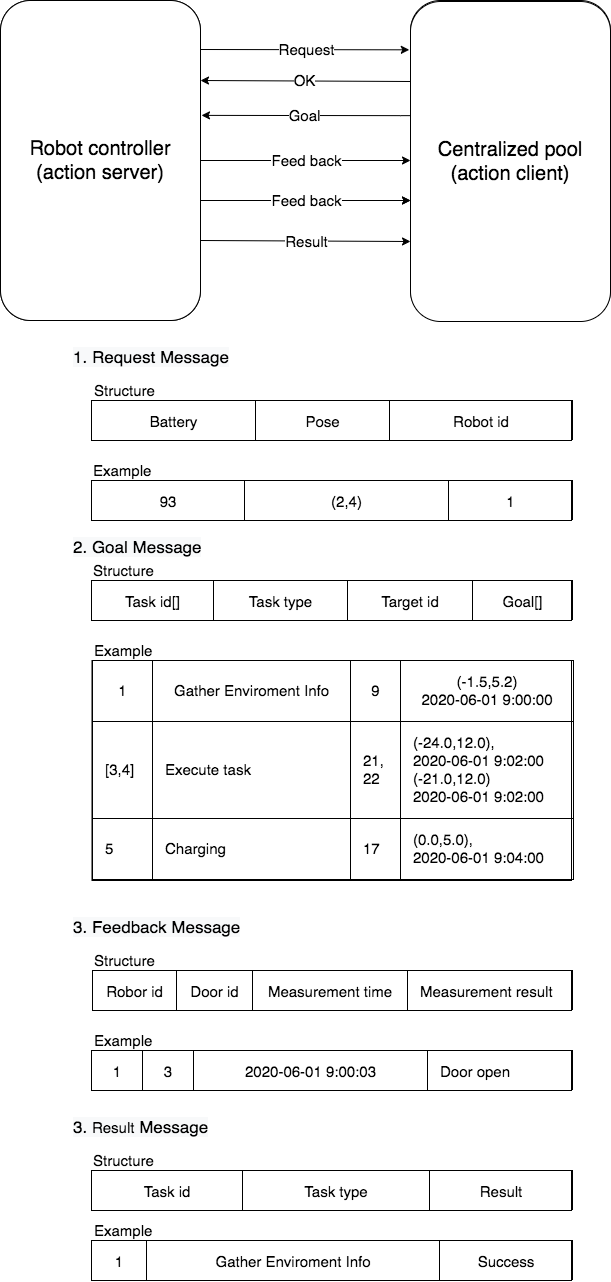
\includegraphics[width = 0.45\textwidth]{content/images/ch3/communication_protocals.drawio.png}
	\caption{Communication Protocols}
	\label{fig:communication_protocals}
\end{figure}

Since centralized pool and robots need to share task information with each other, the communication protocals are required. Four types of message are defined: (1) task request message; (2) task goal messages; (3) task feedback; (4) task result. 
The comparation of task type and examples of each type are shown in Figure \ref{fig:communication_protocals}. 

\section{System Environment}
This section introduce the system enviroment. The 3D module contains a corridor along the central x axis and 16 rooms located around the corridor. The 3D module is shown in Figure \todo{Gazeobo map}  .The 2D map is shown in Figure \ref{fig:room_division}.


\begin{figure}[htbp]
	\centering
	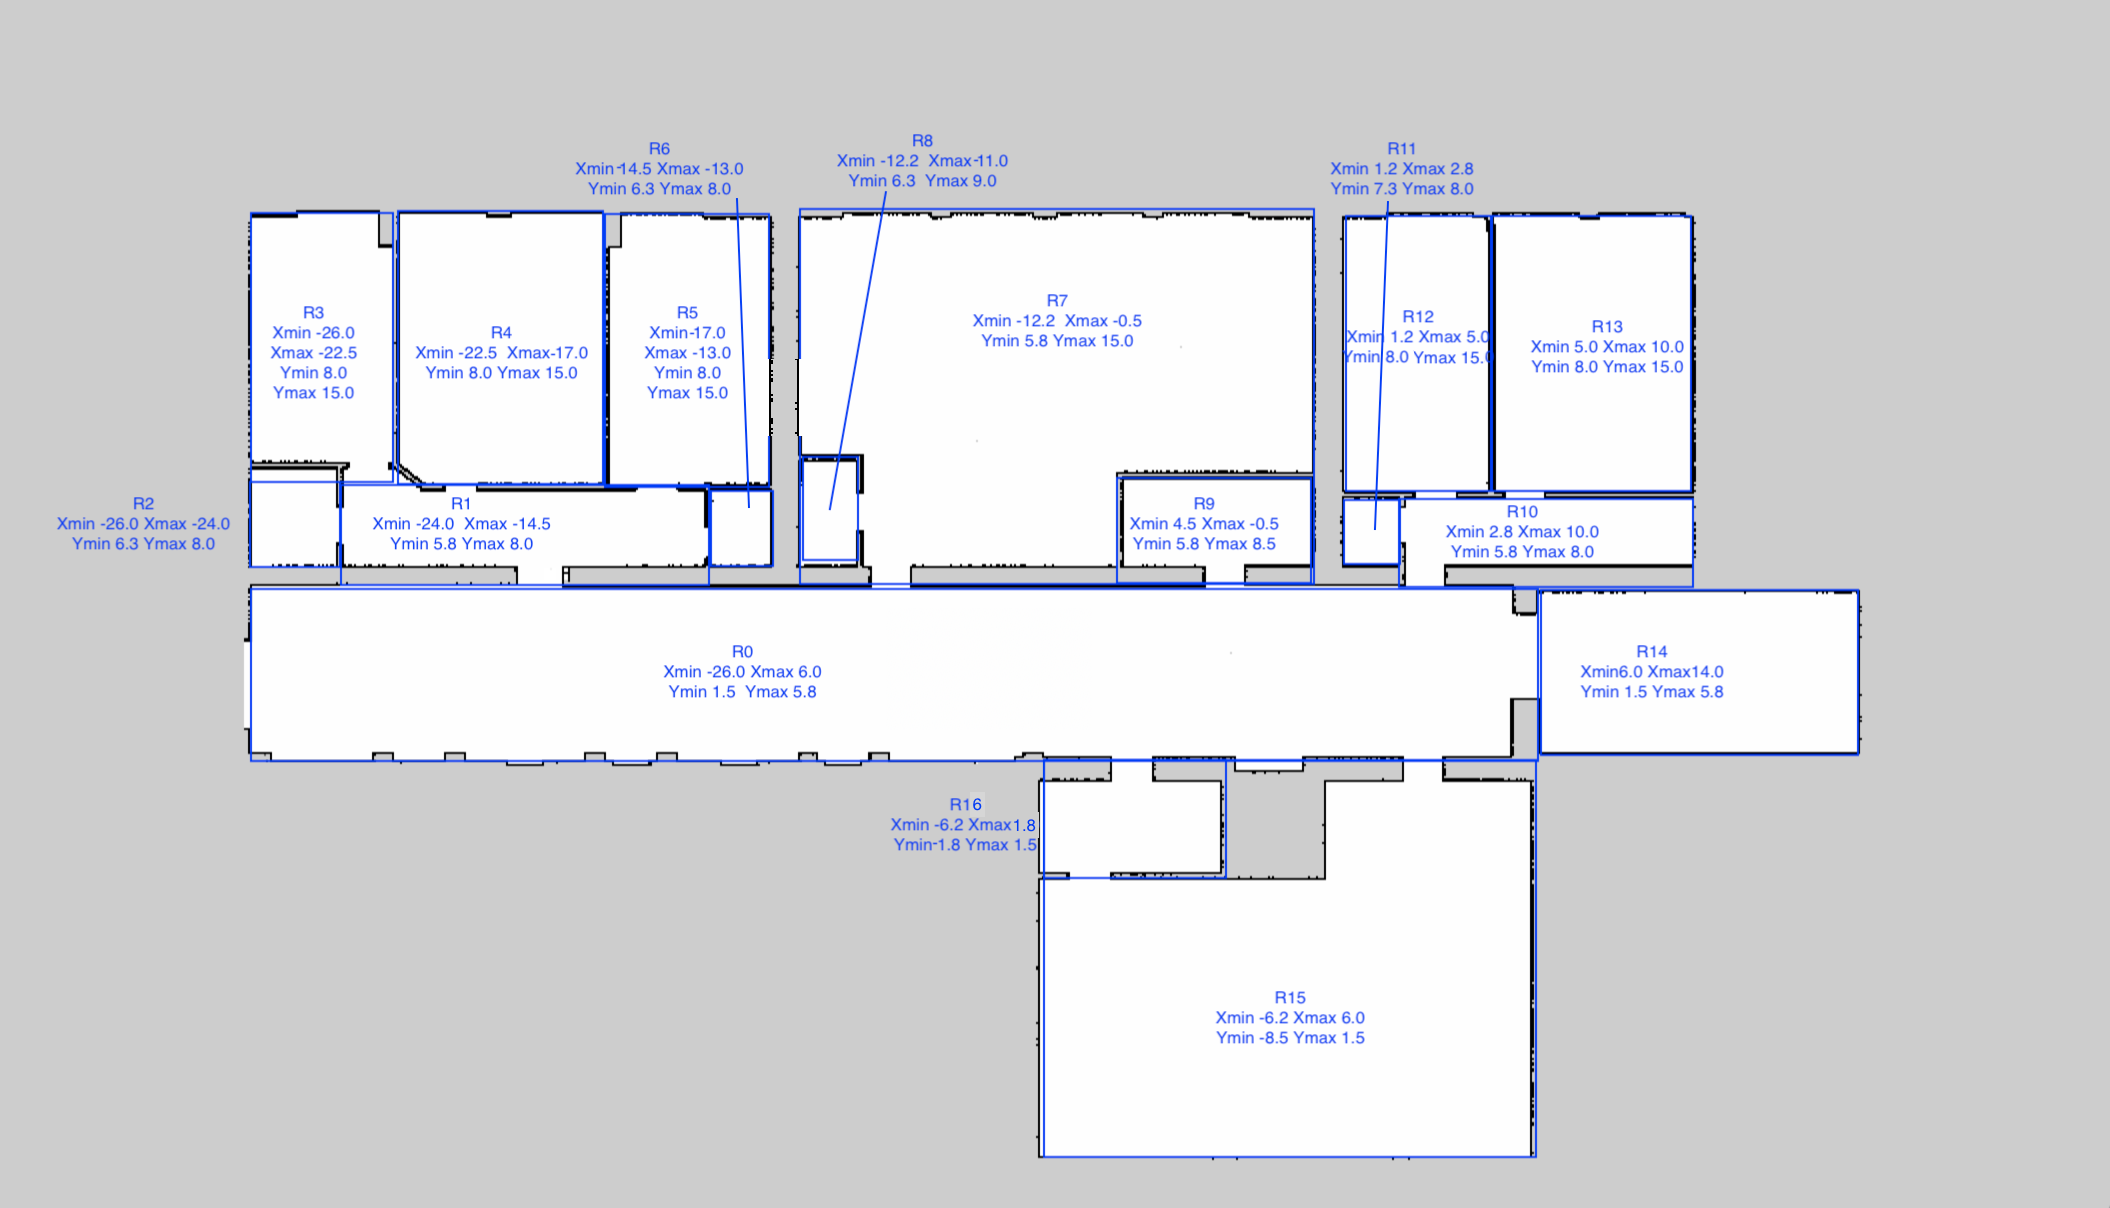
\includegraphics[width = 0.7\textwidth]{content/images/ch3/room_division.png}
	\caption{Room division}
	\label{fig:room_division}
\end{figure}

\subsection{Rooms}
To let the system clearly distinguish which room robot is in, the restrict area(the write area in Figure \ref{fig:room_division}) is divided into rectangles.

\begin{figure}[htbp]
	\centering
	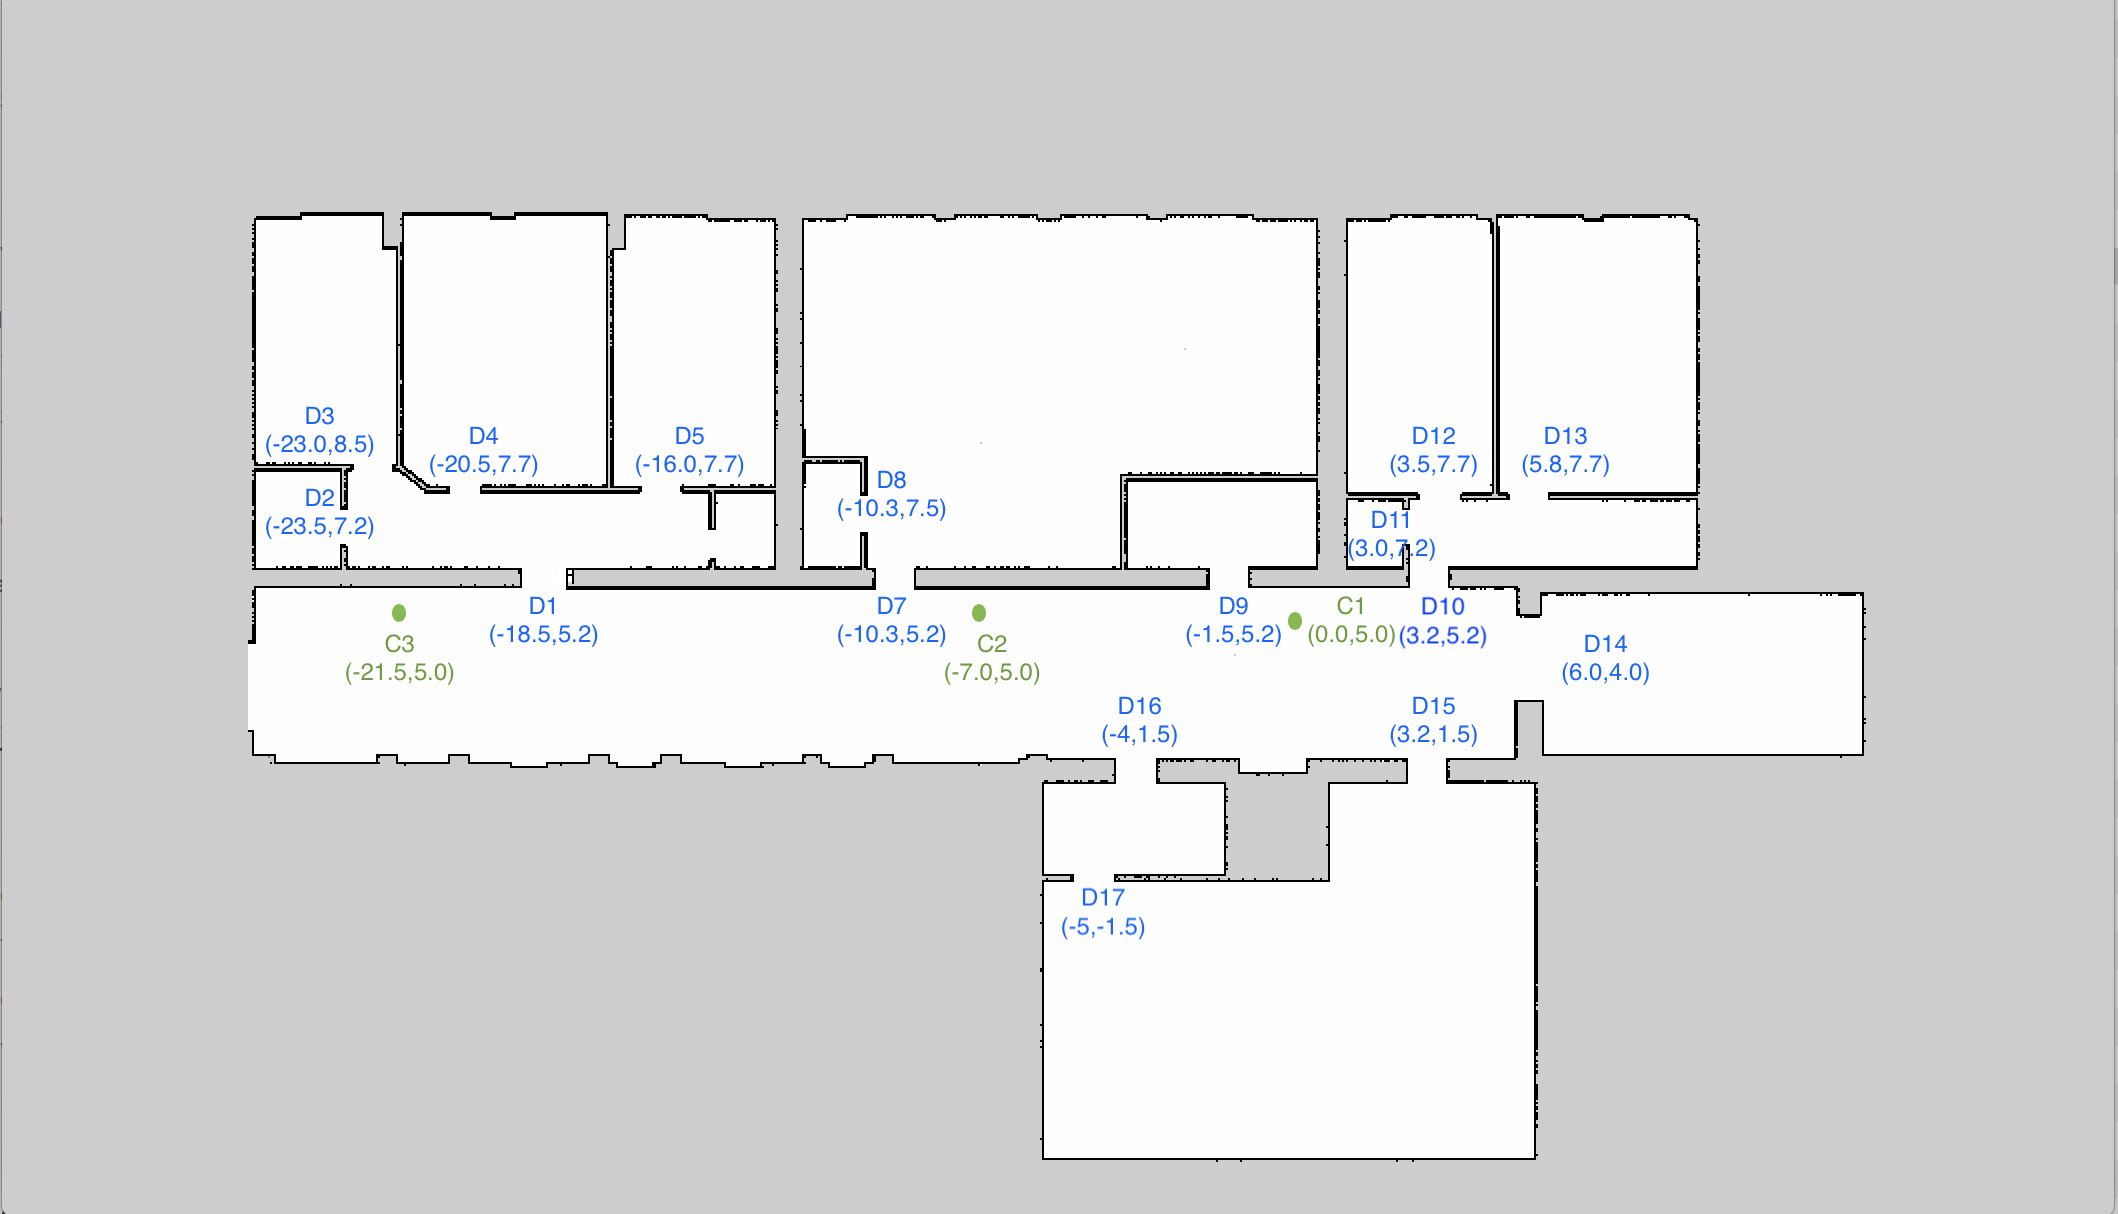
\includegraphics[width = 0.7\textwidth]{content/images/ch3/positions_door_station.png}
	\caption{Doors and Charging Stations}
	\label{fig:positions_door_station}
\end{figure}

\subsection{Doors}
In 3D Model there are no original doors. However in order to simulate an enviroment, a few simulated sensors are created. Those coordinate of sensors are the same as corresponding doors positions (D1-D17 in Figure \ref{fig:positions_door_station}).
Additionally one simulated door sensor is created on the door position. Each simulated door sensors brocasts door status periodically. The broadcast message are received by all robot within its range, including both robots enter the room and robots in corridor passing by the door.
Figure \ref{fig:positions_door_station} shows the distribution of doors.

\subsection{Charging Stations}
The battery decrease is also considered. Three simulated charging stations are located in the corridor. Figure \ref{fig:positions_door_station} shows the distribution of charging stations. 
When robot get a charging task, it would move to one of the charging station and wait until fully charged. The details of robot charging is shown in Section \todo{Robot charging}.

\section{Battery Model}
\label{section:battery_model}

\subsection{Robot battery decrease model}
The decrease amount of robot battery is related to robot trajectory. If a robot get a Large execute task that contains n small task, Equation \ref{eq:battery_consumption} can be used to calculate battery consumption.

\begin{equation}
\begin{aligned}
\label{eq:battery_consumption}
&B: Battery\_Consumption\\
&W: Weight \\
B_{large\_task} & = \sum_{task_0}^{task_n} B_{trajectory} \\
& = \sum_{task_0}^{task_N} \sum_{point_0}^{pont_M} [W_{position} \times position\_variation+W_{angle}  \times angle\_variation]\\
& = \sum_{t = task_0}^{task_N} \sum_{p = point_0}^{point_M} [ W_{position} \times \sqrt{(x_p-x_{p-1} )^2+(y_p-y_{p-1} )^2} \\
&   + W_{angle} \times 2 \times \arccos(w_p)] 
\end{aligned}
\end{equation}

		
\subsection{Recharging model}



\section{Task allocation}

\subsection{Type of task}
\label{sec:task_types}
On one hand, in order to make robot work long hours in office enviroment, recharging is necessary. On the other hand, a robot should gather Enviroment information as much as possible, which centralized pool would learn from and make better decision. 
Therefore, three types of task are defined, which are shown in Table \ref{fig:task_types}. In addition, one single robot is able to carry out one charging task or gather inviroment information task, but can carry multiple execute task, thereby improving overall delivery efficiency. These tasks with dependencies also referred to as small task. Those small tasks form a dependency chain,also referred to as a large task.

%\begin{itemize}
%	\item \textsl{Charging task.} Firstly the robot moves to charging station. Once arrive, the robot send a massage with current battery and wait for a fully charged signal. Other details of robot charging is shown in \todo{Robor charging}
%	\item \textsl{Execute Task.} The robot get
%\end{itemize}

\begin{figure}[htb]
	\centering
	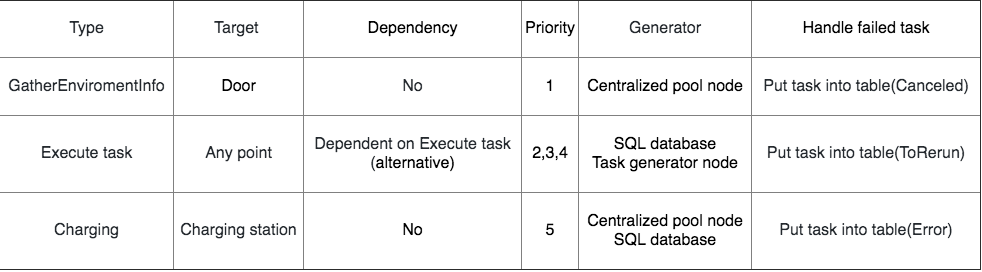
\includegraphics[width = 0.8\textwidth]{content/images/ch3/task_types.drawio.png}
	\caption{Task types}
	\label{fig:task_types}
\end{figure}

\subsection{Cost function}
	A. Cost function for Execute task that contains n small tasks is shown in Equation \ref{eq:large_task_cost}.
\begin{equation}
	\label{eq:large_task_cost}
	\begin{split}
	Cost_{Large\_execute\_task} = \frac{W_{battery} \times Battery\_consum}{n} + W_{waiting} \times Waiting\_time \\
	+ W_{possibility} \times \prod\limits_{i=1}^n Open\_possibility  + W_{priority} \times priority
	\end{split}
\end{equation}
The robot 

 % + wt_wait \times waiting time + \prod\limits_{i=1}^n open possibility+wt_pri × priority
% wt_btr × battery consumption ÷ N + wt_wait × waiting time+ 
\section{Procedure}
The process of 

